\documentclass[conference]{IEEEtran}
\usepackage{graphicx} 						% Haandtering af eksterne billeder (JPG, PNG, EPS, PDF)
\usepackage{multirow}                		% Fletning af raekker og kolonner (\multicolumn og \multirow)
\usepackage{multicol}         	        	% Muliggoer output i spalter
\usepackage{rotating}						% Rotation af tekst med \begin{sideways}...\end{sideways}
\usepackage{colortbl} 						% Farver i tabeller (fx \columncolor og \rowcolor)
\usepackage[table]{xcolor}					% Definer farver med \definecolor. Se mere: http://en.wikibooks.org/wiki/LaTeX/Colors
\usepackage{xcolor}
\usepackage{subcaption}
\usepackage{tikz}
\usetikzlibrary{shapes,arrows,automata,positioning,calc}
\usepackage[utf8]{inputenc}
\usepackage{url}




% Some Computer Society conferences also require the compsoc mode option,
% but others use the standard conference format.
%
% If IEEEtran.cls has not been installed into the LaTeX system files,
% manually specify the path to it like:
% \documentclass[conference]{../sty/IEEEtran}

\usepackage[parfill]{parskip}


% Some very useful LaTeX packages include:
% (uncomment the ones you want to load)


% *** MISC UTILITY PACKAGES ***
%
%\usepackage{ifpdf}
% Heiko Oberdiek's ifpdf.sty is very useful if you need conditional
% compilation based on whether the output is pdf or dvi.
% usage:
% \ifpdf
%   % pdf code
% \else
%   % dvi code
% \fi
% The latest version of ifpdf.sty can be obtained from:
% http://www.ctan.org/pkg/ifpdf
% Also, note that IEEEtran.cls V1.7 and later provides a builtin
% \ifCLASSINFOpdf conditional that works the same way.
% When switching from latex to pdflatex and vice-versa, the compiler may
% have to be run twice to clear warning/error messages.






% *** CITATION PACKAGES ***
%
\usepackage{cite}
% cite.sty was written by Donald Arseneau
% V1.6 and later of IEEEtran pre-defines the format of the cite.sty package
% \cite{} output to follow that of the IEEE. Loading the cite package will
% result in citation numbers being automatically sorted and properly
% "compressed/ranged". e.g., [1], [9], [2], [7], [5], [6] without using
% cite.sty will become [1], [2], [5]--[7], [9] using cite.sty. cite.sty's
% \cite will automatically add leading space, if needed. Use cite.sty's
% noadjust option (cite.sty V3.8 and later) if you want to turn this off
% such as if a citation ever needs to be enclosed in parenthesis.
% cite.sty is already installed on most LaTeX systems. Be sure and use
% version 5.0 (2009-03-20) and later if using hyperref.sty.
% The latest version can be obtained at:
% http://www.ctan.org/pkg/cite
% The documentation is contained in the cite.sty file itself.






% *** GRAPHICS RELATED PACKAGES ***
%
\ifCLASSINFOpdf
  % \usepackage[pdftex]{graphicx}
  % declare the path(s) where your graphic files are
  % \graphicspath{{../pdf/}{../jpeg/}}
  % and their extensions so you won't have to specify these with
  % every instance of \includegraphics
  % \DeclareGraphicsExtensions{.pdf,.jpeg,.png}
\else
  % or other class option (dvipsone, dvipdf, if not using dvips). graphicx
  % will default to the driver specified in the system graphics.cfg if no
  % driver is specified.
  % \usepackage[dvips]{graphicx}
  % declare the path(s) where your graphic files are
  % \graphicspath{{../eps/}}
  % and their extensions so you won't have to specify these with
  % every instance of \includegraphics
  % \DeclareGraphicsExtensions{.eps}
\fi
% graphicx was written by David Carlisle and Sebastian Rahtz. It is
% required if you want graphics, photos, etc. graphicx.sty is already
% installed on most LaTeX systems. The latest version and documentation
% can be obtained at:
% http://www.ctan.org/pkg/graphicx
% Another good source of documentation is "Using Imported Graphics in
% LaTeX2e" by Keith Reckdahl which can be found at:
% http://www.ctan.org/pkg/epslatex
%
% latex, and pdflatex in dvi mode, support graphics in encapsulated
% postscript (.eps) format. pdflatex in pdf mode supports graphics
% in .pdf, .jpeg, .png and .mps (metapost) formats. Users should ensure
% that all non-photo figures use a vector format (.eps, .pdf, .mps) and
% not a bitmapped formats (.jpeg, .png). The IEEE frowns on bitmapped formats
% which can result in "jaggedy"/blurry rendering of lines and letters as
% well as large increases in file sizes.
%
% You can find documentation about the pdfTeX application at:
% http://www.tug.org/applications/pdftex





% *** MATH PACKAGES ***
%
\usepackage{amsmath}
% A popular package from the American Mathematical Society that provides
% many useful and powerful commands for dealing with mathematics.
%
% Note that the amsmath package sets \interdisplaylinepenalty to 10000
% thus preventing page breaks from occurring within multiline equations. Use:
%\interdisplaylinepenalty=2500
% after loading amsmath to restore such page breaks as IEEEtran.cls normally
% does. amsmath.sty is already installed on most LaTeX systems. The latest
% version and documentation can be obtained at:
% http://www.ctan.org/pkg/amsmath





% *** SPECIALIZED LIST PACKAGES ***
%
%\usepackage{algorithmic}
% algorithmic.sty was written by Peter Williams and Rogerio Brito.
% This package provides an algorithmic environment fo describing algorithms.
% You can use the algorithmic environment in-text or within a figure
% environment to provide for a floating algorithm. Do NOT use the algorithm
% floating environment provided by algorithm.sty (by the same authors) or
% algorithm2e.sty (by Christophe Fiorio) as the IEEE does not use dedicated
% algorithm float types and packages that provide these will not provide
% correct IEEE style captions. The latest version and documentation of
% algorithmic.sty can be obtained at:
% http://www.ctan.org/pkg/algorithms
% Also of interest may be the (relatively newer and more customizable)
% algorithmicx.sty package by Szasz Janos:
% http://www.ctan.org/pkg/algorithmicx




% *** ALIGNMENT PACKAGES ***
%
%\usepackage{array}
% Frank Mittelbach's and David Carlisle's array.sty patches and improves
% the standard LaTeX2e array and tabular environments to provide better
% appearance and additional user controls. As the default LaTeX2e table
% generation code is lacking to the point of almost being broken with
% respect to the quality of the end results, all users are strongly
% advised to use an enhanced (at the very least that provided by array.sty)
% set of table tools. array.sty is already installed on most systems. The
% latest version and documentation can be obtained at:
% http://www.ctan.org/pkg/array


% IEEEtran contains the IEEEeqnarray family of commands that can be used to
% generate multiline equations as well as matrices, tables, etc., of high
% quality.




% *** SUBFIGURE PACKAGES ***
%\ifCLASSOPTIONcompsoc
%  \usepackage[caption=false,font=normalsize,labelfont=sf,textfont=sf]{subfig}
%\else
%  \usepackage[caption=false,font=footnotesize]{subfig}
%\fi
% subfig.sty, written by Steven Douglas Cochran, is the modern replacement
% for subfigure.sty, the latter of which is no longer maintained and is
% incompatible with some LaTeX packages including fixltx2e. However,
% subfig.sty requires and automatically loads Axel Sommerfeldt's caption.sty
% which will override IEEEtran.cls' handling of captions and this will result
% in non-IEEE style figure/table captions. To prevent this problem, be sure
% and invoke subfig.sty's "caption=false" package option (available since
% subfig.sty version 1.3, 2005/06/28) as this is will preserve IEEEtran.cls
% handling of captions.
% Note that the Computer Society format requires a larger sans serif font
% than the serif footnote size font used in traditional IEEE formatting
% and thus the need to invoke different subfig.sty package options depending
% on whether compsoc mode has been enabled.
%
% The latest version and documentation of subfig.sty can be obtained at:
% http://www.ctan.org/pkg/subfig




% *** FLOAT PACKAGES ***
%
%\usepackage{fixltx2e}
% fixltx2e, the successor to the earlier fix2col.sty, was written by
% Frank Mittelbach and David Carlisle. This package corrects a few problems
% in the LaTeX2e kernel, the most notable of which is that in current
% LaTeX2e releases, the ordering of single and double column floats is not
% guaranteed to be preserved. Thus, an unpatched LaTeX2e can allow a
% single column figure to be placed prior to an earlier double column
% figure.
% Be aware that LaTeX2e kernels dated 2015 and later have fixltx2e.sty's
% corrections already built into the system in which case a warning will
% be issued if an attempt is made to load fixltx2e.sty as it is no longer
% needed.
% The latest version and documentation can be found at:
% http://www.ctan.org/pkg/fixltx2e


%\usepackage{stfloats}
% stfloats.sty was written by Sigitas Tolusis. This package gives LaTeX2e
% the ability to do double column floats at the bottom of the page as well
% as the top. (e.g., "\begin{figure*}[!b]" is not normally possible in
% LaTeX2e). It also provides a command:
%\fnbelowfloat
% to enable the placement of footnotes below bottom floats (the standard
% LaTeX2e kernel puts them above bottom floats). This is an invasive package
% which rewrites many portions of the LaTeX2e float routines. It may not work
% with other packages that modify the LaTeX2e float routines. The latest
% version and documentation can be obtained at:
% http://www.ctan.org/pkg/stfloats
% Do not use the stfloats baselinefloat ability as the IEEE does not allow
% \baselineskip to stretch. Authors submitting work to the IEEE should note
% that the IEEE rarely uses double column equations and that authors should try
% to avoid such use. Do not be tempted to use the cuted.sty or midfloat.sty
% packages (also by Sigitas Tolusis) as the IEEE does not format its papers in
% such ways.
% Do not attempt to use stfloats with fixltx2e as they are incompatible.
% Instead, use Morten Hogholm'a dblfloatfix which combines the features
% of both fixltx2e and stfloats:
%
% \usepackage{dblfloatfix}
% The latest version can be found at:
% http://www.ctan.org/pkg/dblfloatfix




% *** PDF, URL AND HYPERLINK PACKAGES ***
%
%\usepackage{url}
% url.sty was written by Donald Arseneau. It provides better support for
% handling and breaking URLs. url.sty is already installed on most LaTeX
% systems. The latest version and documentation can be obtained at:
% http://www.ctan.org/pkg/url
% Basically, \url{my_url_here}.


\usepackage{todonotes}

% nomenclature
  \usepackage{nomencl}
  \makenomenclature
  \setlength{\nomlabelwidth}{1cm}
  \setlength{\nomitemsep}{-\parsep}

% *** Do not adjust lengths that control margins, column widths, etc. ***
% *** Do not use packages that alter fonts (such as pslatex).         ***
% There should be no need to do such things with IEEEtran.cls V1.6 and later.
% (Unless specifically asked to do so by the journal or conference you plan
% to submit to, of course. )



% correct bad hyphenation here
\hyphenation{op-tical net-works semi-conduc-tor}


\begin{document}
 \nomenclature{MIS}{Minimal invasive surgery}
 \nomenclature{RMIS}{Robotic minimal invasive surgery}
 \nomenclature{ROS}{Robots operating system}
 \nomenclature{DOF}{Degrees of freedom}




 


% paper title
% Titles are generally capitalized except for words such as a, an, and, as,
% at, but, by, for, in, nor, of, on, or, the, to and up, which are usually
% not capitalized unless they are the first or last word of the title.
% Linebreaks \\ can be used within to get better formatting as desired.
% Do not put math or special symbols in the title.
\graphicspath{ {../Worksheets/rapport/pictures/} }
%%% Tikz Magic %%%


\tikzstyle{block} = [draw, fill=blue!20, rectangle, minimum height=3em, minimum width=6em]
\tikzstyle{Integrator} = [draw, fill=blue!20, rectangle, minimum height=5mm, minimum width=5mm]
\tikzstyle{Twolineblock} = [draw, fill=blue!20, rectangle, minimum height=3em, minimum width=6em, text width = 6em, align=center]       
\tikzstyle{sum} = [draw, fill=blue!20, circle, node distance=1cm]
\tikzstyle{input} = [coordinate]
\tikzstyle{output} = [coordinate]
\tikzstyle{pinstyle} = [pin edge={to-,thin,black}]
\tikzstyle{box} = [draw,rounded corners, minimum height=15mm, minimum width=20mm, align=center, text centered]
\tikzstyle{BlackBox} = [draw, fill=black, rounded corners, minimum height=15mm, minimum width=20mm, align=center, text=white, text centered]
\tikzstyle{FlowIF} = [diamond, draw, fill=blue!20, text width=8.5em, text badly centered, node distance=3cm, inner sep=0pt,align=center,aspect=3]
\tikzstyle{FlowBlock} = [rectangle, draw, fill=blue!20, text width=8em, text centered, rounded corners, minimum height=3em]
\tikzstyle{FlowCloud} = [draw, ellipse,fill=black!40!red,box, node distance=3cm, minimum height=2em]
\tikzstyle{TestBox} = [rectangle,draw, fill=black!20, minimum height=8mm, minimum width=8mm]
\tikzstyle{TestDiamond} = [diamond, draw, fill=black!20, aspect=2, minimum height=8mm]
%\tikzstyle{TestDiamond} = [diamond, draw, fill=black!20, minimum height=5mm, minimum width=5mm]

\tikzstyle{TestBox} = [rectangle,draw, fill=black!20, minimum height=8mm, minimum width=8mm]
\tikzstyle{TestCircle} = [circle, draw, fill=black!20, minimum height=6mm, minimum width=6mm]
\tikzstyle{TestTable} = [rectangle, draw, fill=black!60, minimum height=0.01mm, minimum width=9mm, text=white]
\tikzstyle{TestBoxSmall} = [rectangle,draw, fill=black!, minimum height=8mm, minimum width=8mm,text=white]
\tikzstyle{LegendBox} = [rectangle,draw, minimum height=7mm, minimum width=20mm]
\tikzstyle{Sysbox} = [draw,rounded corners, minimum height=15mm, minimum width=9em, align=center, text centered,text width = 10.5em]
\tikzstyle{SysBlackBox} = [draw, fill=black, text=white, rounded corners, minimum height=15mm, minimum width=9em, align=center, text centered,text width = 10em]


\title{Teleoperation of surgical robot using force feedback}


% author names and affiliations
% use a multiple column layout for up to three different
% affiliations
\author{\IEEEauthorblockN{Daniel Bolgar}
\and
\IEEEauthorblockN{Simon Krogh}
\and
\IEEEauthorblockN{Filip Marić}
\and
\IEEEauthorblockN{Nicolas Silvani}
}

% conference papers do not typically use \thanks and this command
% is locked out in conference mode. If really needed, such as for
% the acknowledgment of grants, issue a \IEEEoverridecommandlockouts
% after \documentclass

% for over three affiliations, or if they all won't fit within the width
% of the page, use this alternative format:
%
%\author{\IEEEauthorblockN{Michael Shell\IEEEauthorrefmark{1},
%Homer Simpson\IEEEauthorrefmark{2},
%James Kirk\IEEEauthorrefmark{3},
%Montgomery Scott\IEEEauthorrefmark{3} and
%Eldon Tyrell\IEEEauthorrefmark{4}}
%\IEEEauthorblockA{\IEEEauthorrefmark{1}School of Electrical and Computer Engineering\\
%Georgia Institute of Technology,
%Atlanta, Georgia 30332--0250\\ Email: see http://www.michaelshell.org/contact.html}
%\IEEEauthorblockA{\IEEEauthorrefmark{2}Twentieth Century Fox, Springfield, USA\\
%Email: homer@thesimpsons.com}
%\IEEEauthorblockA{\IEEEauthorrefmark{3}Starfleet Academy, San Francisco, California 96678-2391\\
%Telephone: (800) 555--1212, Fax: (888) 555--1212}
%\IEEEauthorblockA{\IEEEauthorrefmark{4}Tyrell Inc., 123 Replicant Street, Los Angeles, California 90210--4321}}




% use for special paper notices
%\IEEEspecialpapernotice{(Invited Paper)}




% make the title area
\maketitle

% As a general rule, do not put math, special symbols or citations
% in the abstract
\begin{abstract}

Haptic feedback is a form of transferring information to the user via the sense of touch, usually through some sort of input device the user gives commands with.
This makes it ideal for teleoperating tasks requiring precision in applied force, robotic surgery being a prime example.
Currently, haptic feedback in teleoperation is subject to numerous constraints on time delay and accuracy.
Nonetheless, results show that implementing this type of feedback in teleoperated robotic surgery gives vastly better results.
In this paper we propose a new method of teleoperating the DaVinci surgical robot using haptic feedback.
The method involves using a state-of-the-art haptic device to control a surgical tool serving as the robots end-effector.
Since the dynamics of the surgical tool are strongly non-linear, estimation techniques are used to calculate reaction forces on the device.
Changes are made to existing communication protocols in order to reduce time delay\todo{Maybe add results (operating frequency for example)}, which is an important factor.
The various constraints and challenges are adressed individually in each section. \todo{Erase last sentence}
\end{abstract}
% no keywords
\hfill August 26, 2015

\printnomenclature

% For peer review papers, you can put extra information on the cover
% page as needed:
% \ifCLASSOPTIONpeerreview
% \begin{center} \bfseries EDICS Category: 3-BBND \end{center}
% \fi
%
% For peerreview papers, this IEEEtran command inserts a page break and
% creates the second title. It will be ignored for other modes.
\IEEEpeerreviewmaketitle

\section{Introduction}
% no \IEEEPARstart
Over the last couple of decades the use of robots for minimally invasive surgeries has increased.
This is mainly due to its precision and the reduction in tissue damage\cite{RIGSP}.
Robots used in these surgical procedures have an attached end-effector that is used as a surgical tool.
One such tool is the Endowrist. 
The main advantage of the Endowrist lies in its construction, as it is made to be manipulated in a similar manner to a human wrist.

Currently the only feedback operators get is visual, using live video transmissions of the surgery. 
The problem with the operator having exclusively visual feedback lies in the fact that the surgeon has to estimate the force applied by the deformation of the skin and organs for each maneuver. %to skin and organs in every single manoeuvre made. 
It has been shown experimentally that haptic feedback has a considerably positive effect on the reduction in surgical error\cite{EOFGFF}. 

The purpose of haptic feedback is to apply force that resist the operators movement in such a way that it represents some information about the environment or situation.
In theory, this should make teleoperated surgical procedures a lot more realistic to the operator and thus reduce accidents.

The haptic feedback could be done as direct force feedback calculated from the resistance on the actuators but as the tool is highly non-linear the transparency of the controller will become less transparent\todo{transparent x2}.
It would be possible to solve this problem by implementing a sensor to the end effector to measure the force but due to the demand of high hygiene the tools have to be sterilized at temperatures over a $100^\circ$ C which could damage the sensor(s). Furthermore it is stated by law that each surgical tool has to be discarded after a few times in use\todo{after a few use}. This means that the cost of the tool has to stay as low as possible and therefore make the idea of implementing an expensive sensor not ideal.

Therefore the force feedback has to be estimated through the actuators which gives a high demand for the feedback controller as it has to be as precise as possible to feedback the correct force to the operator. Another important subject is the transparency of the feedback as the operator should have the feeling of doing the operation by hand and not remote\todo{remotely or through a robot}. This puts a demand on the speed of the feedback loop as the faster the loop runs the more smooth the force feedback to the operator will feel. This will set demands on communication frequency since we need to keep time delay to a minimum. It is wildly discussed what the minimum refresh rate of the feedback loop should be but seems to be someplace between 300 Hz and a\todo{remove "a"} 1000 Hz\cite{coles2011role}. 

In the section II we will take an overview of our proposed control system as a whole, briefly presenting each of the components and their interaction.
Section III will cover methods used to create a dynamic model of the Endowrist and proposed methods of translating the estimated force to actual force fed back to the operator.
Section IV contains descriptions of various problems pertaining the requirement of transparency and explanations of methods used to address them.
Finally,  we present (the expected) experimental results in section V and and draw a short conclusion in section VI.
 
 \section{System overview}
In out\todo{our?} proposed system, the surgeon uses the Geomagic Touch joystick to control an Endowrist tool on one of the arms of the DaVinci surgical robot.
It is important for the operator to have a feeling of resistance the tool is experiencing in order to adjust the position and grip strength and thus prevent damage to the patients tissue.
To achieve this, we use the Geomagics haptic feedback feature in order to project the reaction forces acting on the Endowrist to the operator. 
The communication between system components is done through the Robot Operating System (ROS).

\subsection{Endowrist}
An Endowrist, see \ref{fig:Endo_plates} \todo{figref?} is a surgical tool which can be manipulated as a human wrist. 
It is used in surgical procedures such as Laparoscopic surgeries, better known as minimally invasive surgery (MIS), where small incisions in the human body is made during the surgery. 
Because the incision cuts are small, blood lose\todo{blood loss?} during the surgery and the risk of infection is reduced. This has a positive effect on the recovery time for the patient.

\begin{figure}
	\centering
	\begin{subfigure}{.22\textwidth}
		\centering
		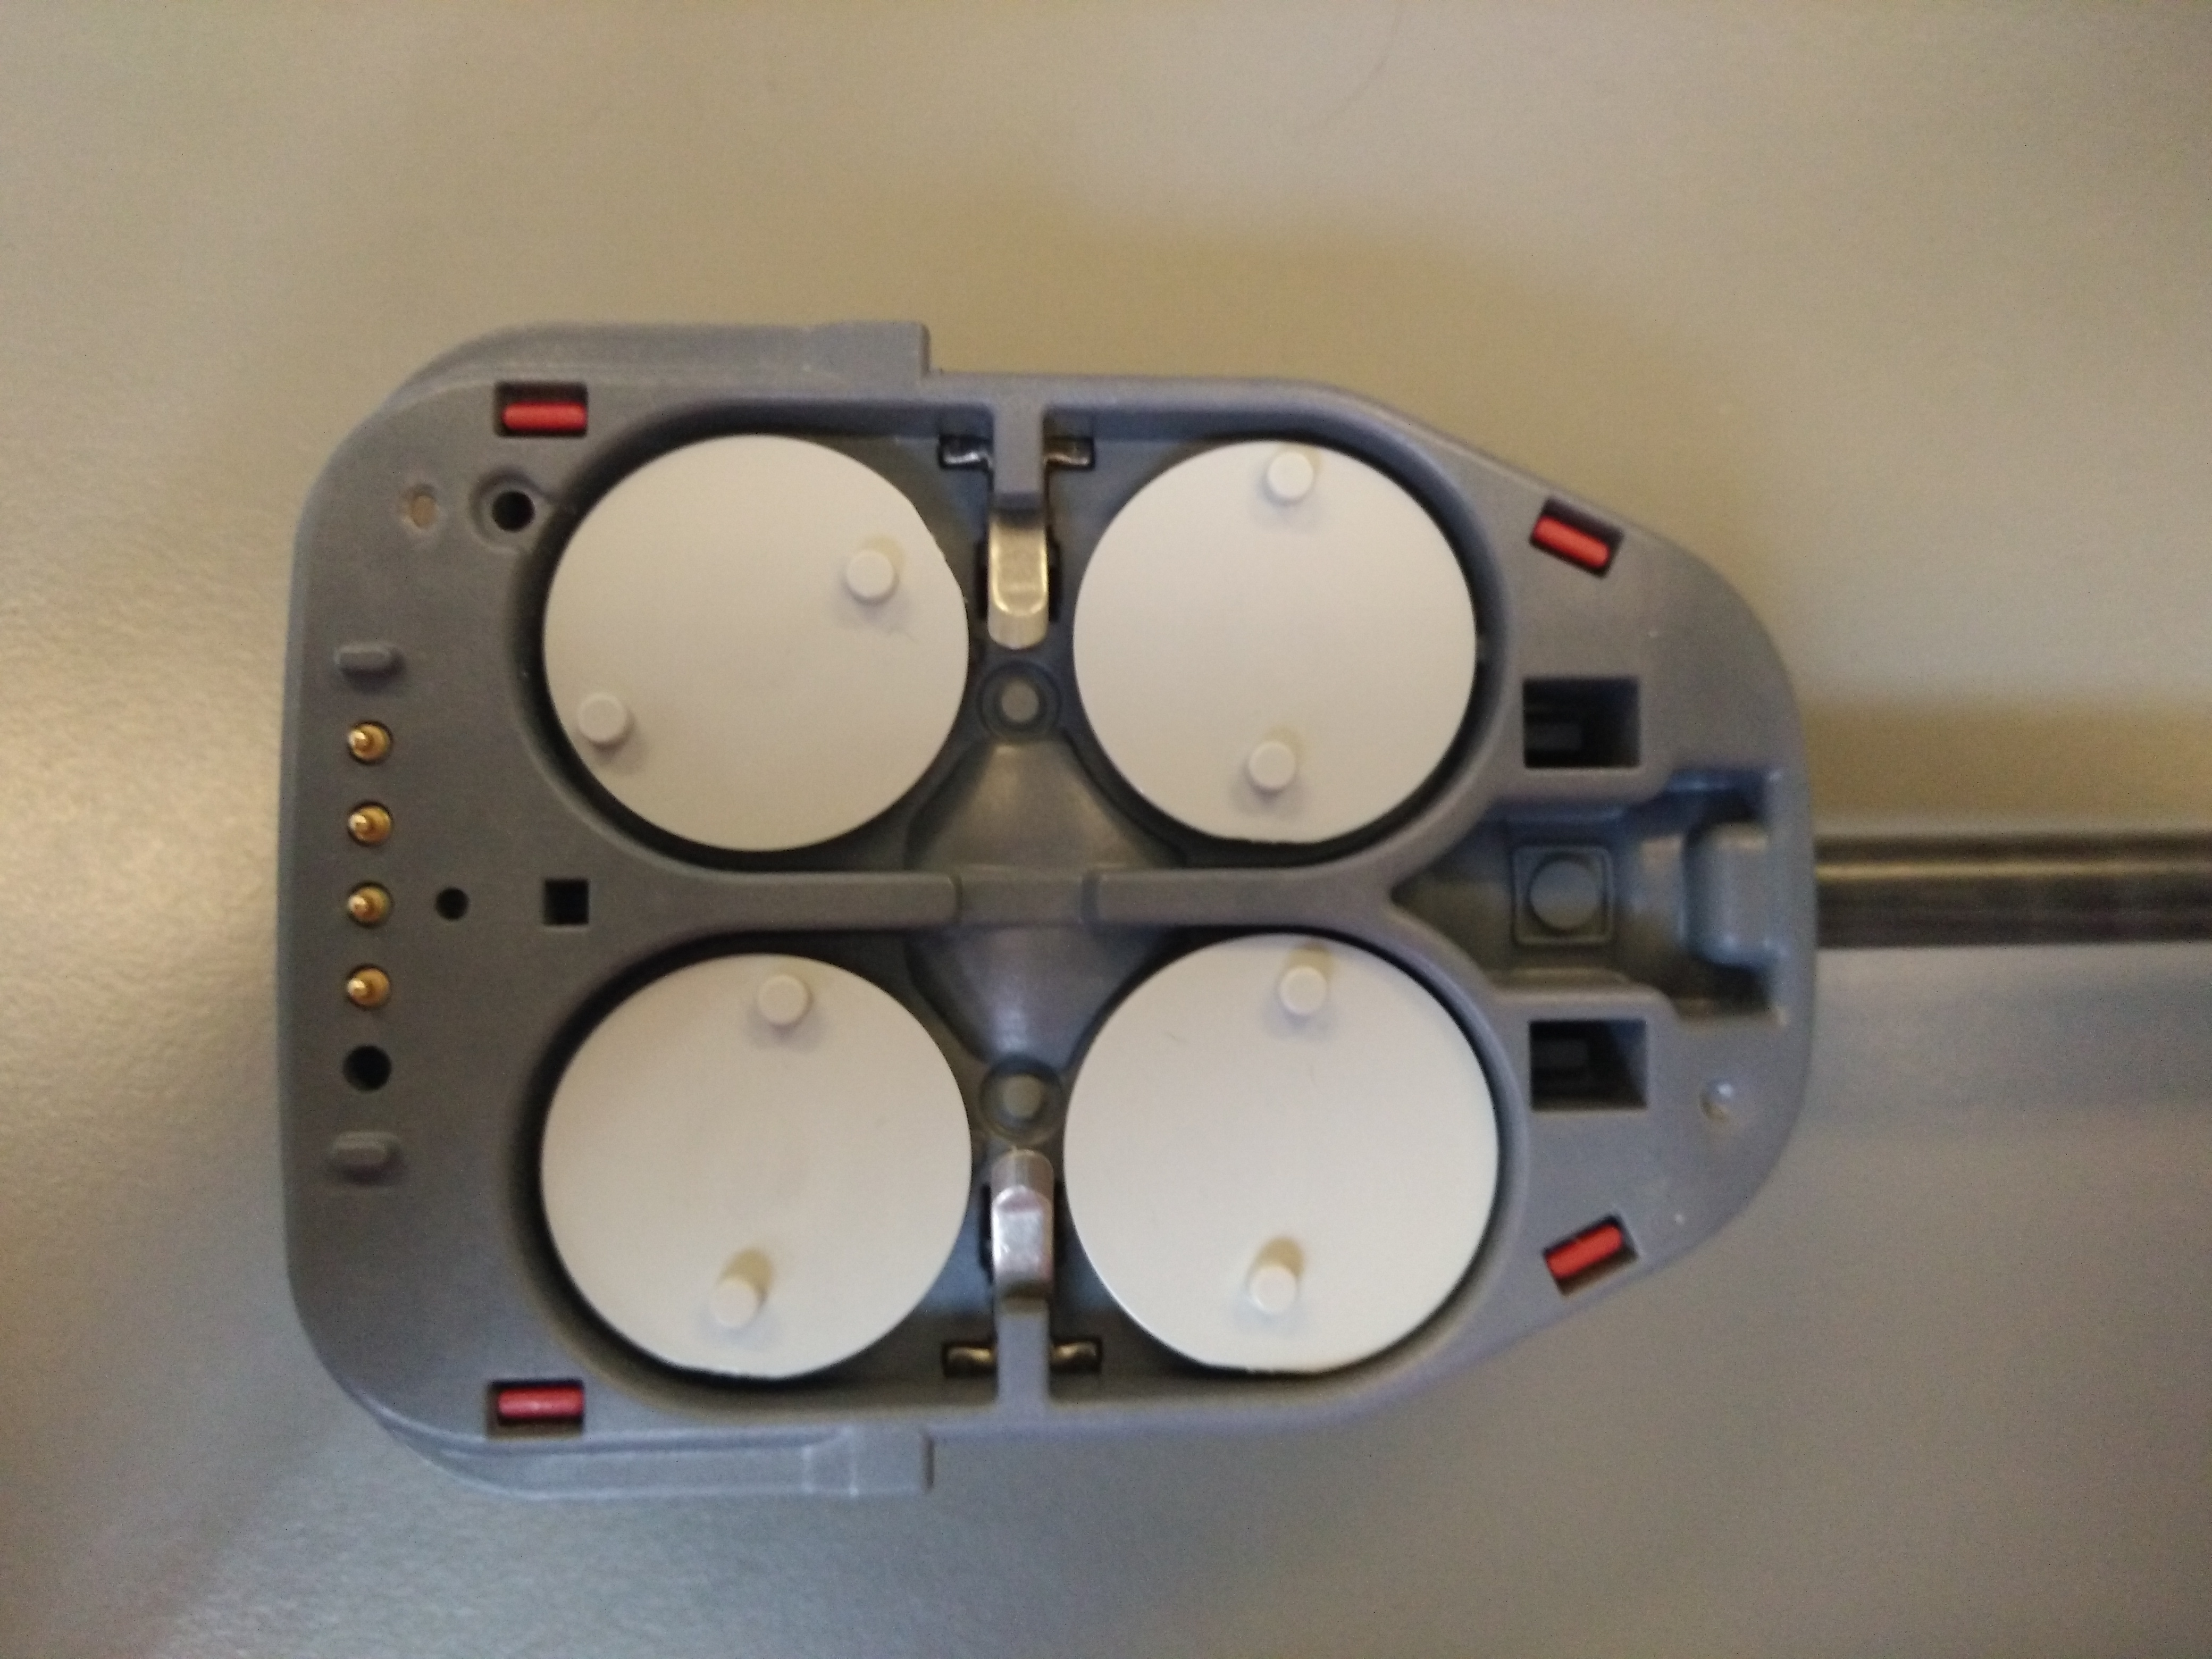
\includegraphics[width=\linewidth]{Endowrist2.jpg}
		\caption{Actuator plates, which can alternate the end effector position}
		\label{fig:Endo_plates}
	\end{subfigure}
	\begin{subfigure}{.22\textwidth}
		\centering
		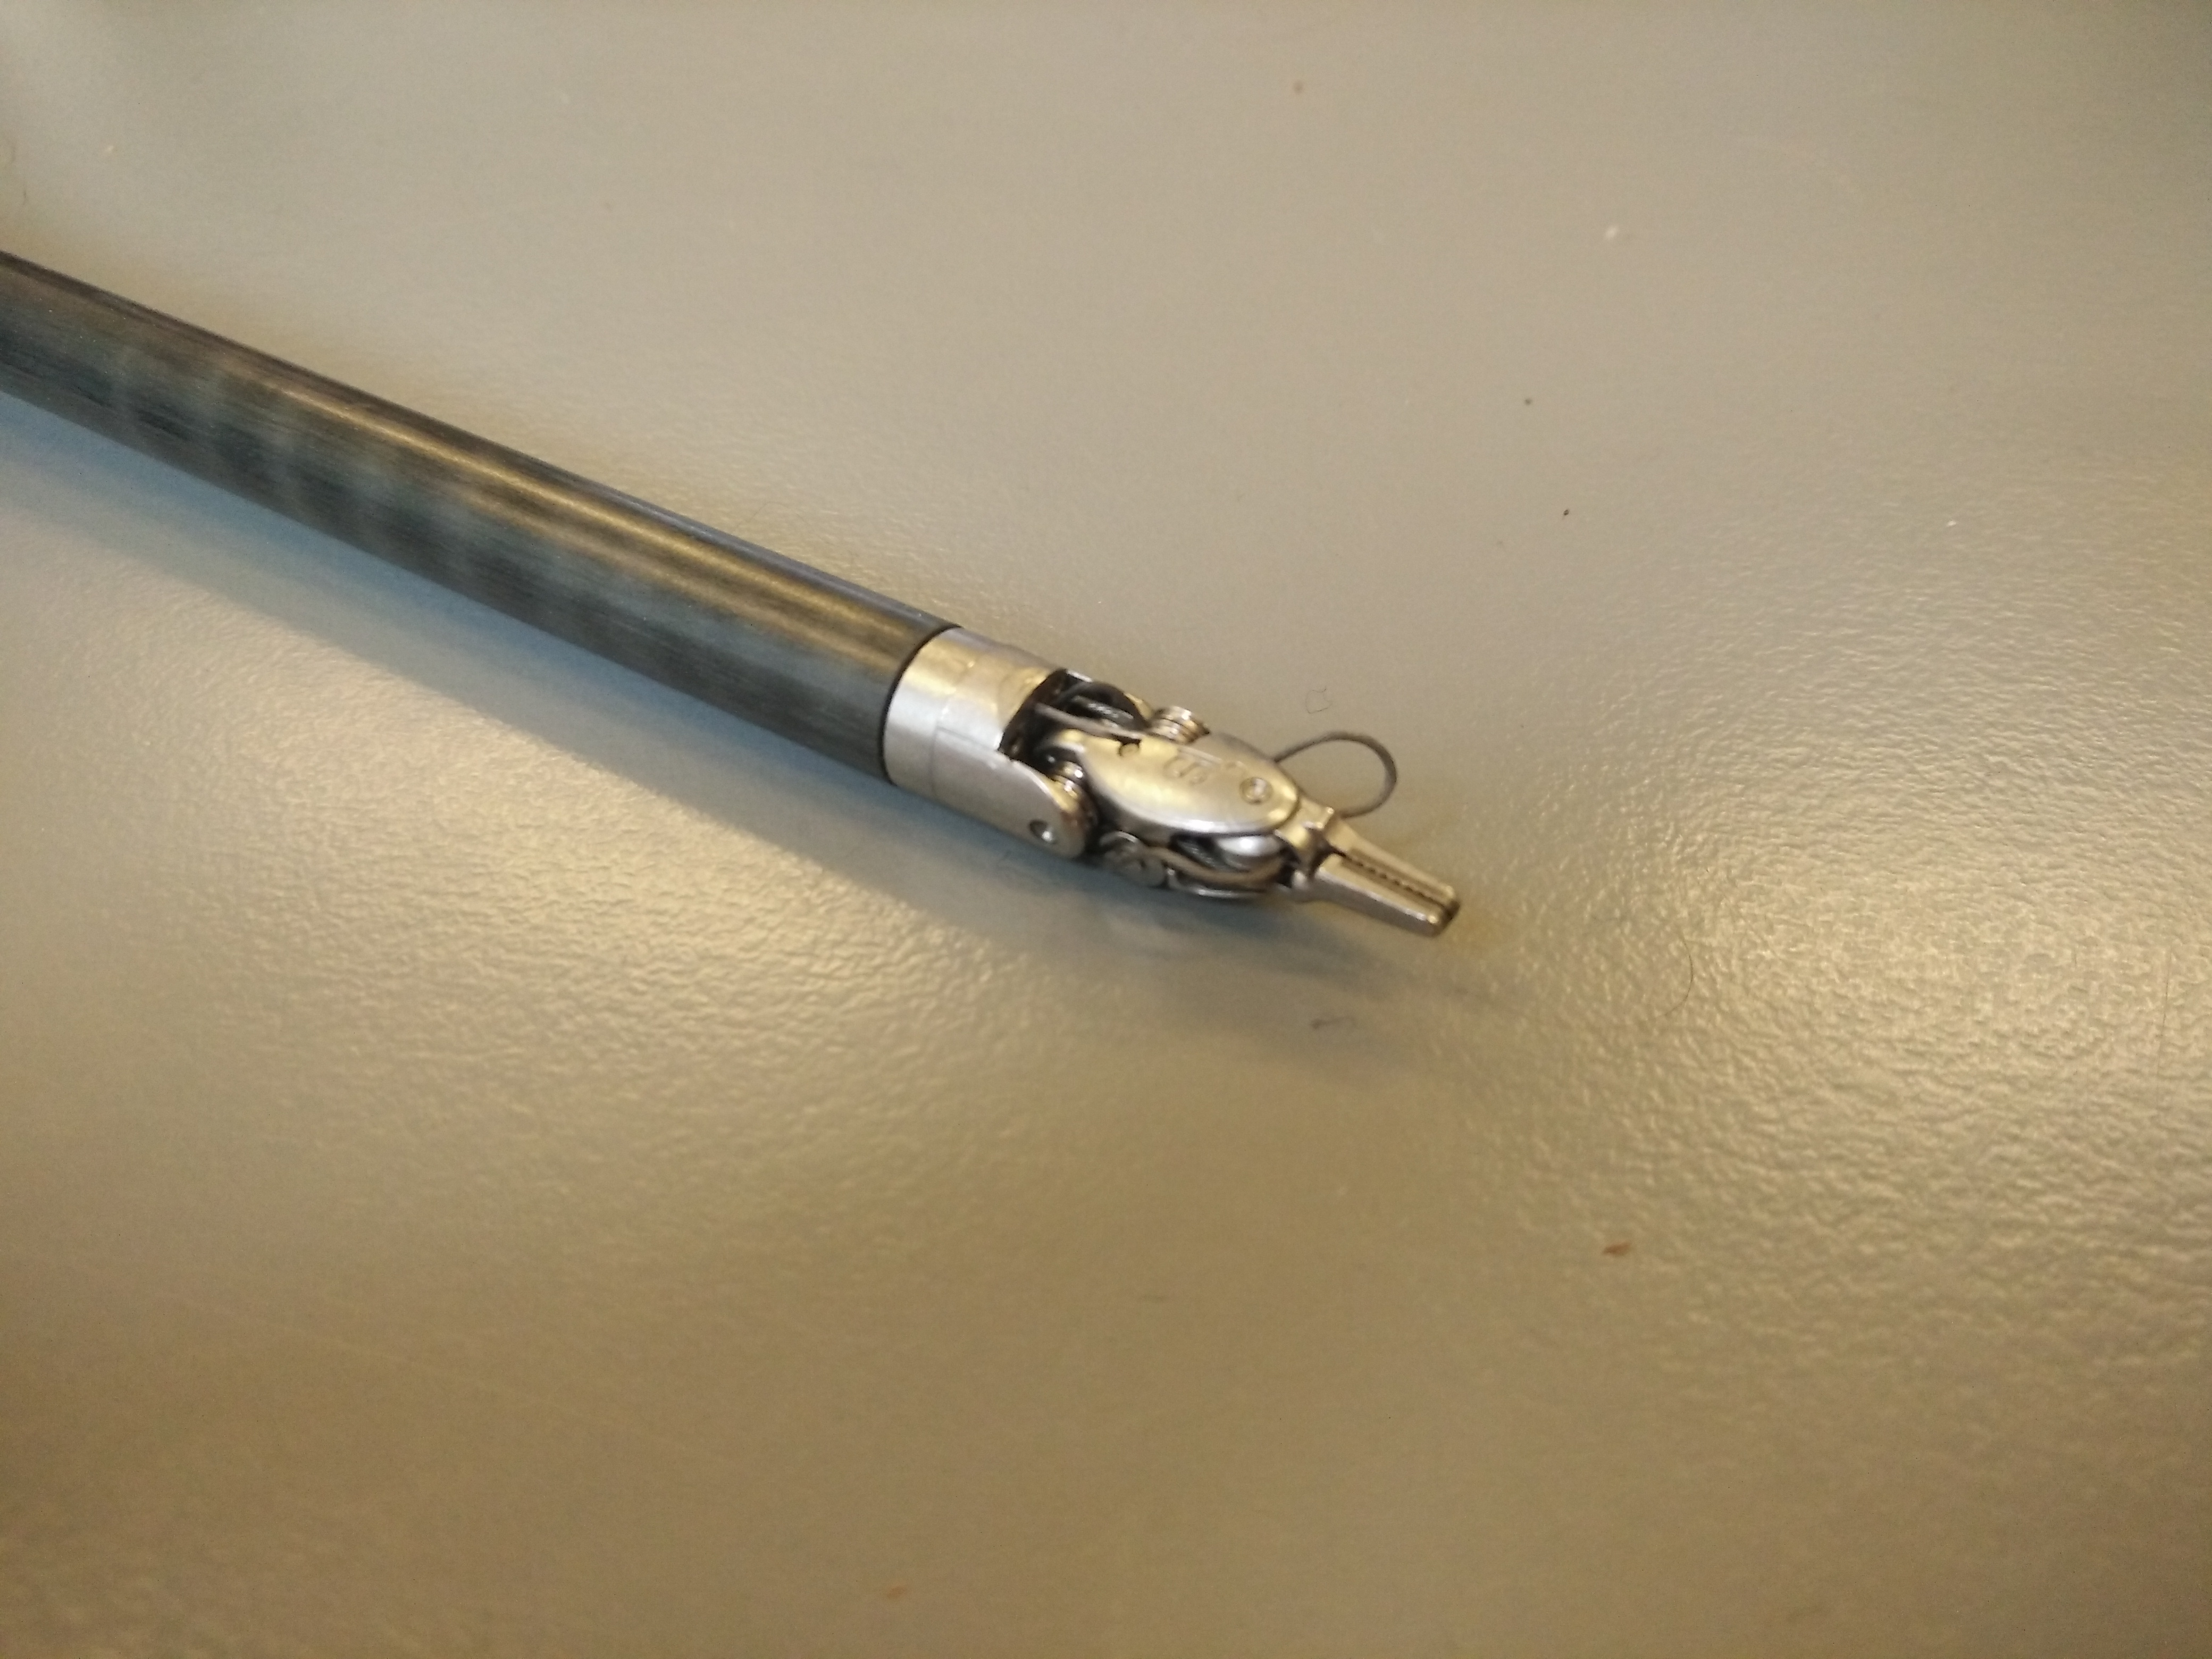
\includegraphics[width=\linewidth]{Endowrist3.jpg}
		\caption{End effector of the Endowrist\newline}
		\label{fig:Endo_end}
	\end{subfigure}
\caption{The Endowrist and it's end-effector}
\label{fig:endowrits_set}
\end{figure}

As mentioned the Endowrist has the ability to be manipulated as a human wrist and thereby has four DOF, see \ref{fig:Endo_end}\todo{1b doesn't really show the 4DOF}\todo{figref}. This enables the movement of roll, pitch, yaw and an open closing mechanism that acts as the thumb and index finger of a hand. 

The end-effector is manipulated by the four wheels seen on \ref{fig:Endo_plates}. Wheel one and three define the movement of the yaw and the closing mechanism. Wheel two and four moves the pitch and roll. The Endowrist is cable driven, which enables the opportunity of making the Endowrist small but it also makes the system nonlinear as the force acting at one end is not directly transmitted to the other end due to friction. 

\subsection{Geomagic touch}
The geomagic touch is a haptic feedback device, which has the ability to manipulate its joints in such a way that the user feels resistance when moving the pen in a certain direction or way. 
The geomagic touch described in this section is the model Phantom omni and can be seen on \ref{fig:phantom_omni}.

\begin{figure}
	\centering
	\begin{subfigure}{.22\textwidth}
		\centering
		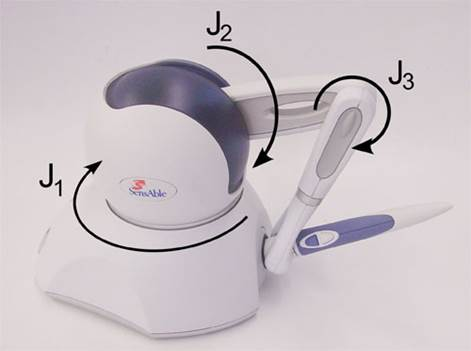
\includegraphics[width=\linewidth]{haptick1.jpg}
		\caption{Overview of the Phantom omni's first three joints.}
		\label{fig:phantom1}
	\end{subfigure}
	\begin{subfigure}{.22\textwidth}
		\centering
		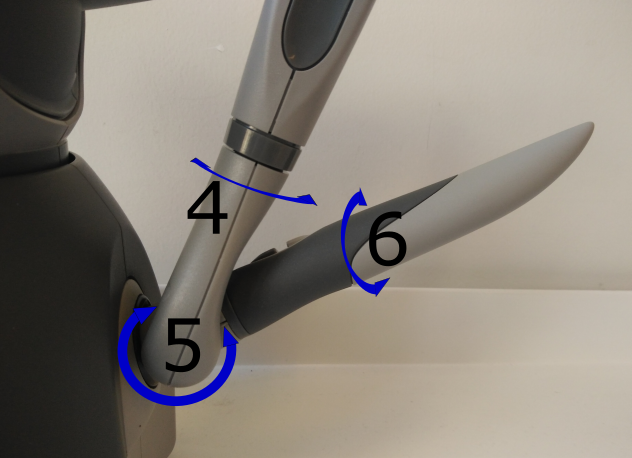
\includegraphics[width=\linewidth]{haptick2.png}
		\caption{Overview of the Phantom omni's last three joint}
		\label{fig:phantom2}
	\end{subfigure}
\caption{Overview of all the Phantom omni's joints\cite{phantom_omni}}
\label{fig:phantom_omni}
\end{figure}

As mentioned the Phantom omni has the ability to generate resistance for the user. In other words, when moved in a specific direction it can create a counter force in respect to a certain position. On \ref{fig:phantom_omni}, it can be seen that the omni has six DOF, where only the first three can be actuated, see \ref{fig:phantom1}. This means that the device only has the ability to generate force feedback with three DOF, in this case roll, pitch and yaw.

The connection to the omni can either be made directly through a ethernet cable or through ethernet cable to a usb converter into a computer. For programming the omni an API is included, which enables the connection to the omni. The Geomagic Touch has a lot of features which can be programmed through the language C++, e.g force rendering or drawing graphics.

\subsection{ROS} \todo{we should not describe what ROS is}
The ROS is an open source software development tool for implementing robotics software. It provides the opportunity of hardware abstraction, low level device control, implementation of commonly used functionalities, messages between different processes and package management.%{\cite{wiki_ros}}
 It provides tools and libraries which utilize the the opportunity of communicating between disturbed computers, obtaining, writing and running codes.
 
ROS has three different levels of concepts\cite{Wiki_ros_concepts}

\begin{itemize}
\item \textbf{The file system level}

Handles the main unit for a ROS system which is packages. A package may include data sets, ROS dependent libraries, configure files etc. to define a ROS process. In ROS a process is denoted as a node. 
\item \textbf{The computation graph level}

Handles the communication of the peer to peer network of the system in which data is processed. Through the computation graph level, the different nodes can communicate with each other by messages. When a node is sending data it is said to be publishing a topic. The different nodes can then subscribe to this topic to get the information that is published.
\item \textbf{The Community level}

ROS has a huge community which contain distribution of software installations, repositories and documentation of ROS. It also has a question and answer section with ROS related topics.
This community makes the process of learning the system considerably easier.
\end{itemize}

\subsection{Overview}
As mentioned before , a fully featured DaVinci robot \todo{arm} has 7 degrees of freedom on the Endowrist instrument.
Since the robot has 4 arms, there are 4 instruments.
Although our setup controls only 4 motors, in funcionality it is equivalent to one DaVinci arm. \todo{I find this confusing}

\begin{figure}
		\centering
		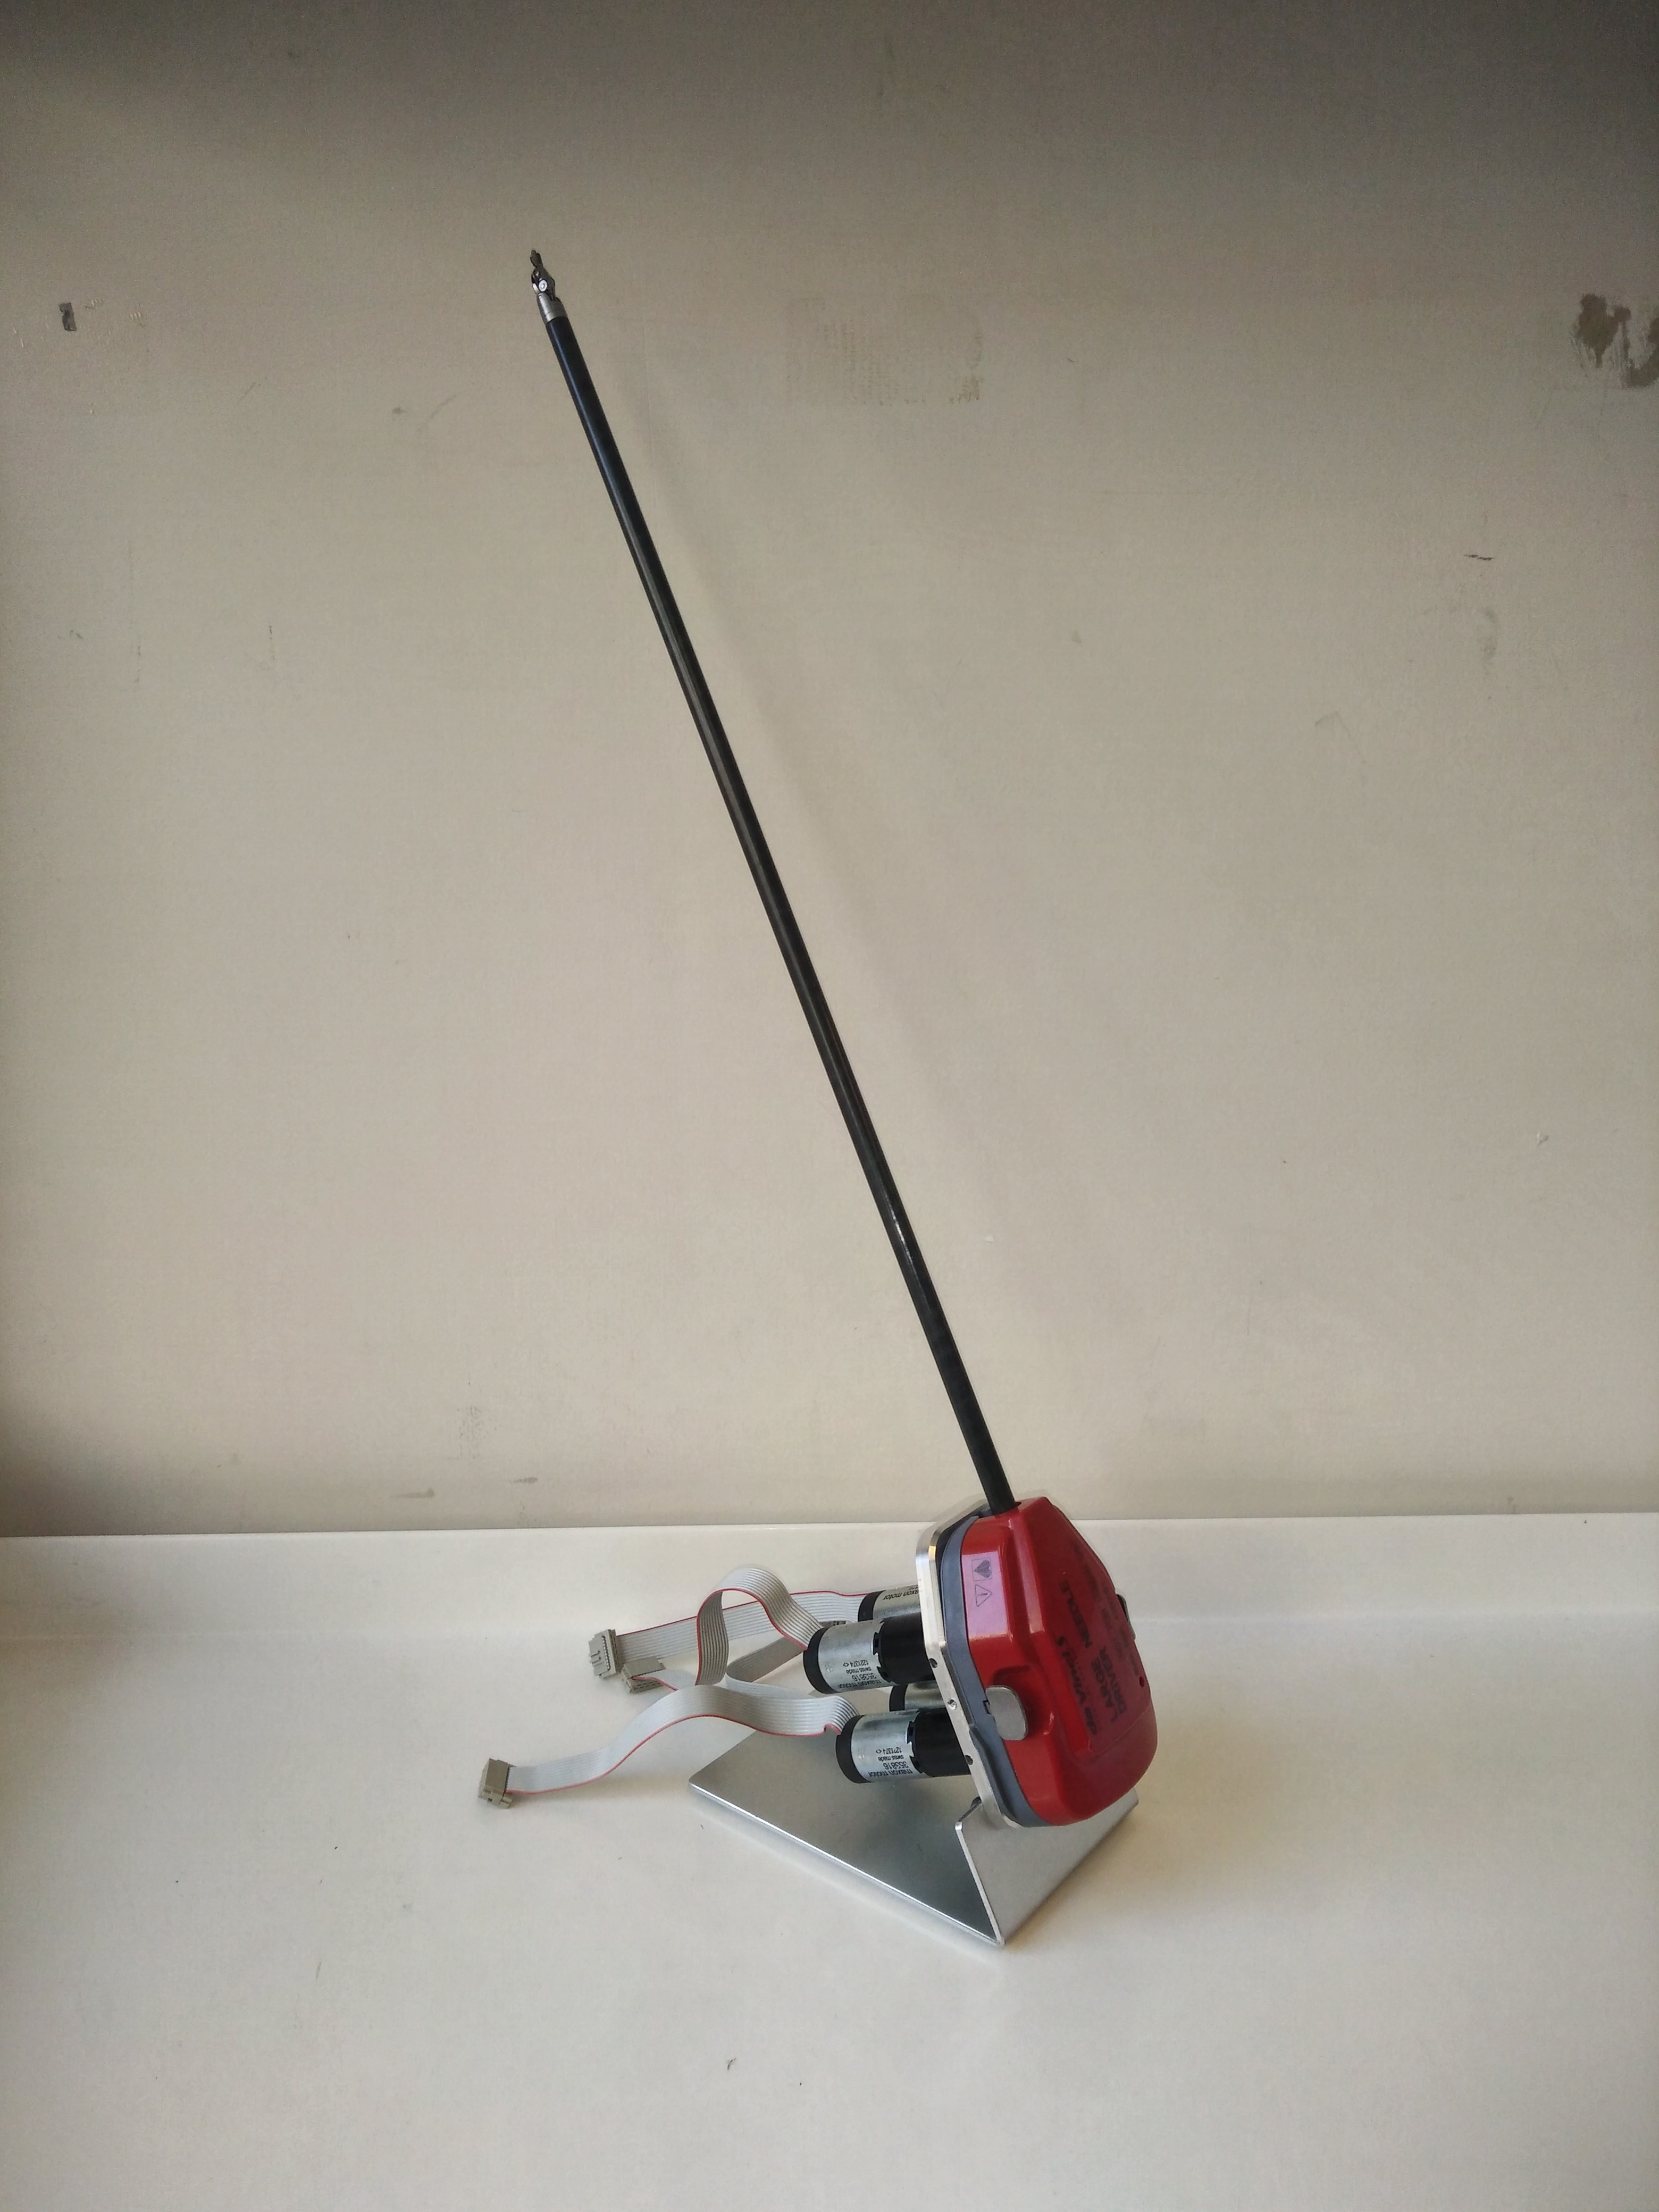
\includegraphics[width=0.4\linewidth]{Test_setup4.jpg}
		\caption{Full view of the mechanical test setup}
		\label{fig:Mec_d}
\end{figure}

As mentioned before, the sbRio board controls the test setup and as such represents the onboard computer on the DaVinci robot.
In order to perform higher level functions such as force feedback control, it is necessary to remotely handle data and send high-level commands.
This is handled by an external computer system that is connected to the Phantom omni device.

The sbRio board communicates with the computer using UDP \todo{UDP is one of our results and not part of the initial setup} communication protocols, while the Geomagic Touch does so using TCP/IP.
The computer also performs force estimation using a dynamical model of the test setup (or Endowrist, more precisely), this is vital for force feedback.
In order to connect software components responsible for communicating with hardware and the ones responsible for the control algorithm and estimation.
For this purpose we use the Robot Operating System (ROS), which uses a network architecture to share data between components via data streams.

\begin{figure}[h]
\centering
\begin{tikzpicture}
    % We start by placing the blocks
    \node [block] (Geomagic) {\small{Geomagic Touch}};
    \node [block, right of=Geomagic, node distance = 3.4cm] (ROS) {ROS};
    \node [block, right of=ROS, node distance=3.3cm] (DaVinci) {DaVinci};
    % We draw an edge between the controller and system block to 
    % calculate the coordinate u. We need it to place the measurement block. 
    \draw [<->] (Geomagic) -- node[label=above:\small{TCP/IP}] {} (ROS);
    \draw [<->] (ROS) -- node [label=above:\small{UDP}] {} (DaVinci);
\end{tikzpicture}
\caption{Block diagram representing the system.}
\end{figure}

\section{Force estimation}
In order to have a representation of the reaction force on the Endowrist, we must resort to estimation.
Because of the reasons mentioned in section II, we cannot measure it directly using sensors and thus have to rely on mathematical models as functions of torque measurements.

\subsection{Mathematical model}
The main challenge we face in making a model lies in the fact that the pulley system on the Endowrist is non-linear, and thus its full dynamics cannot be modeled in a simple manner.
Regardless, a physical model for grip force can be derived \cite{kim2014dynamic}, which serves as a good starting point for parameter estimation.
This model only calculates grip force, which we consider acceptable since it is the arguably the most important variable to feedback to the operator.
\begin{figure}
\centering
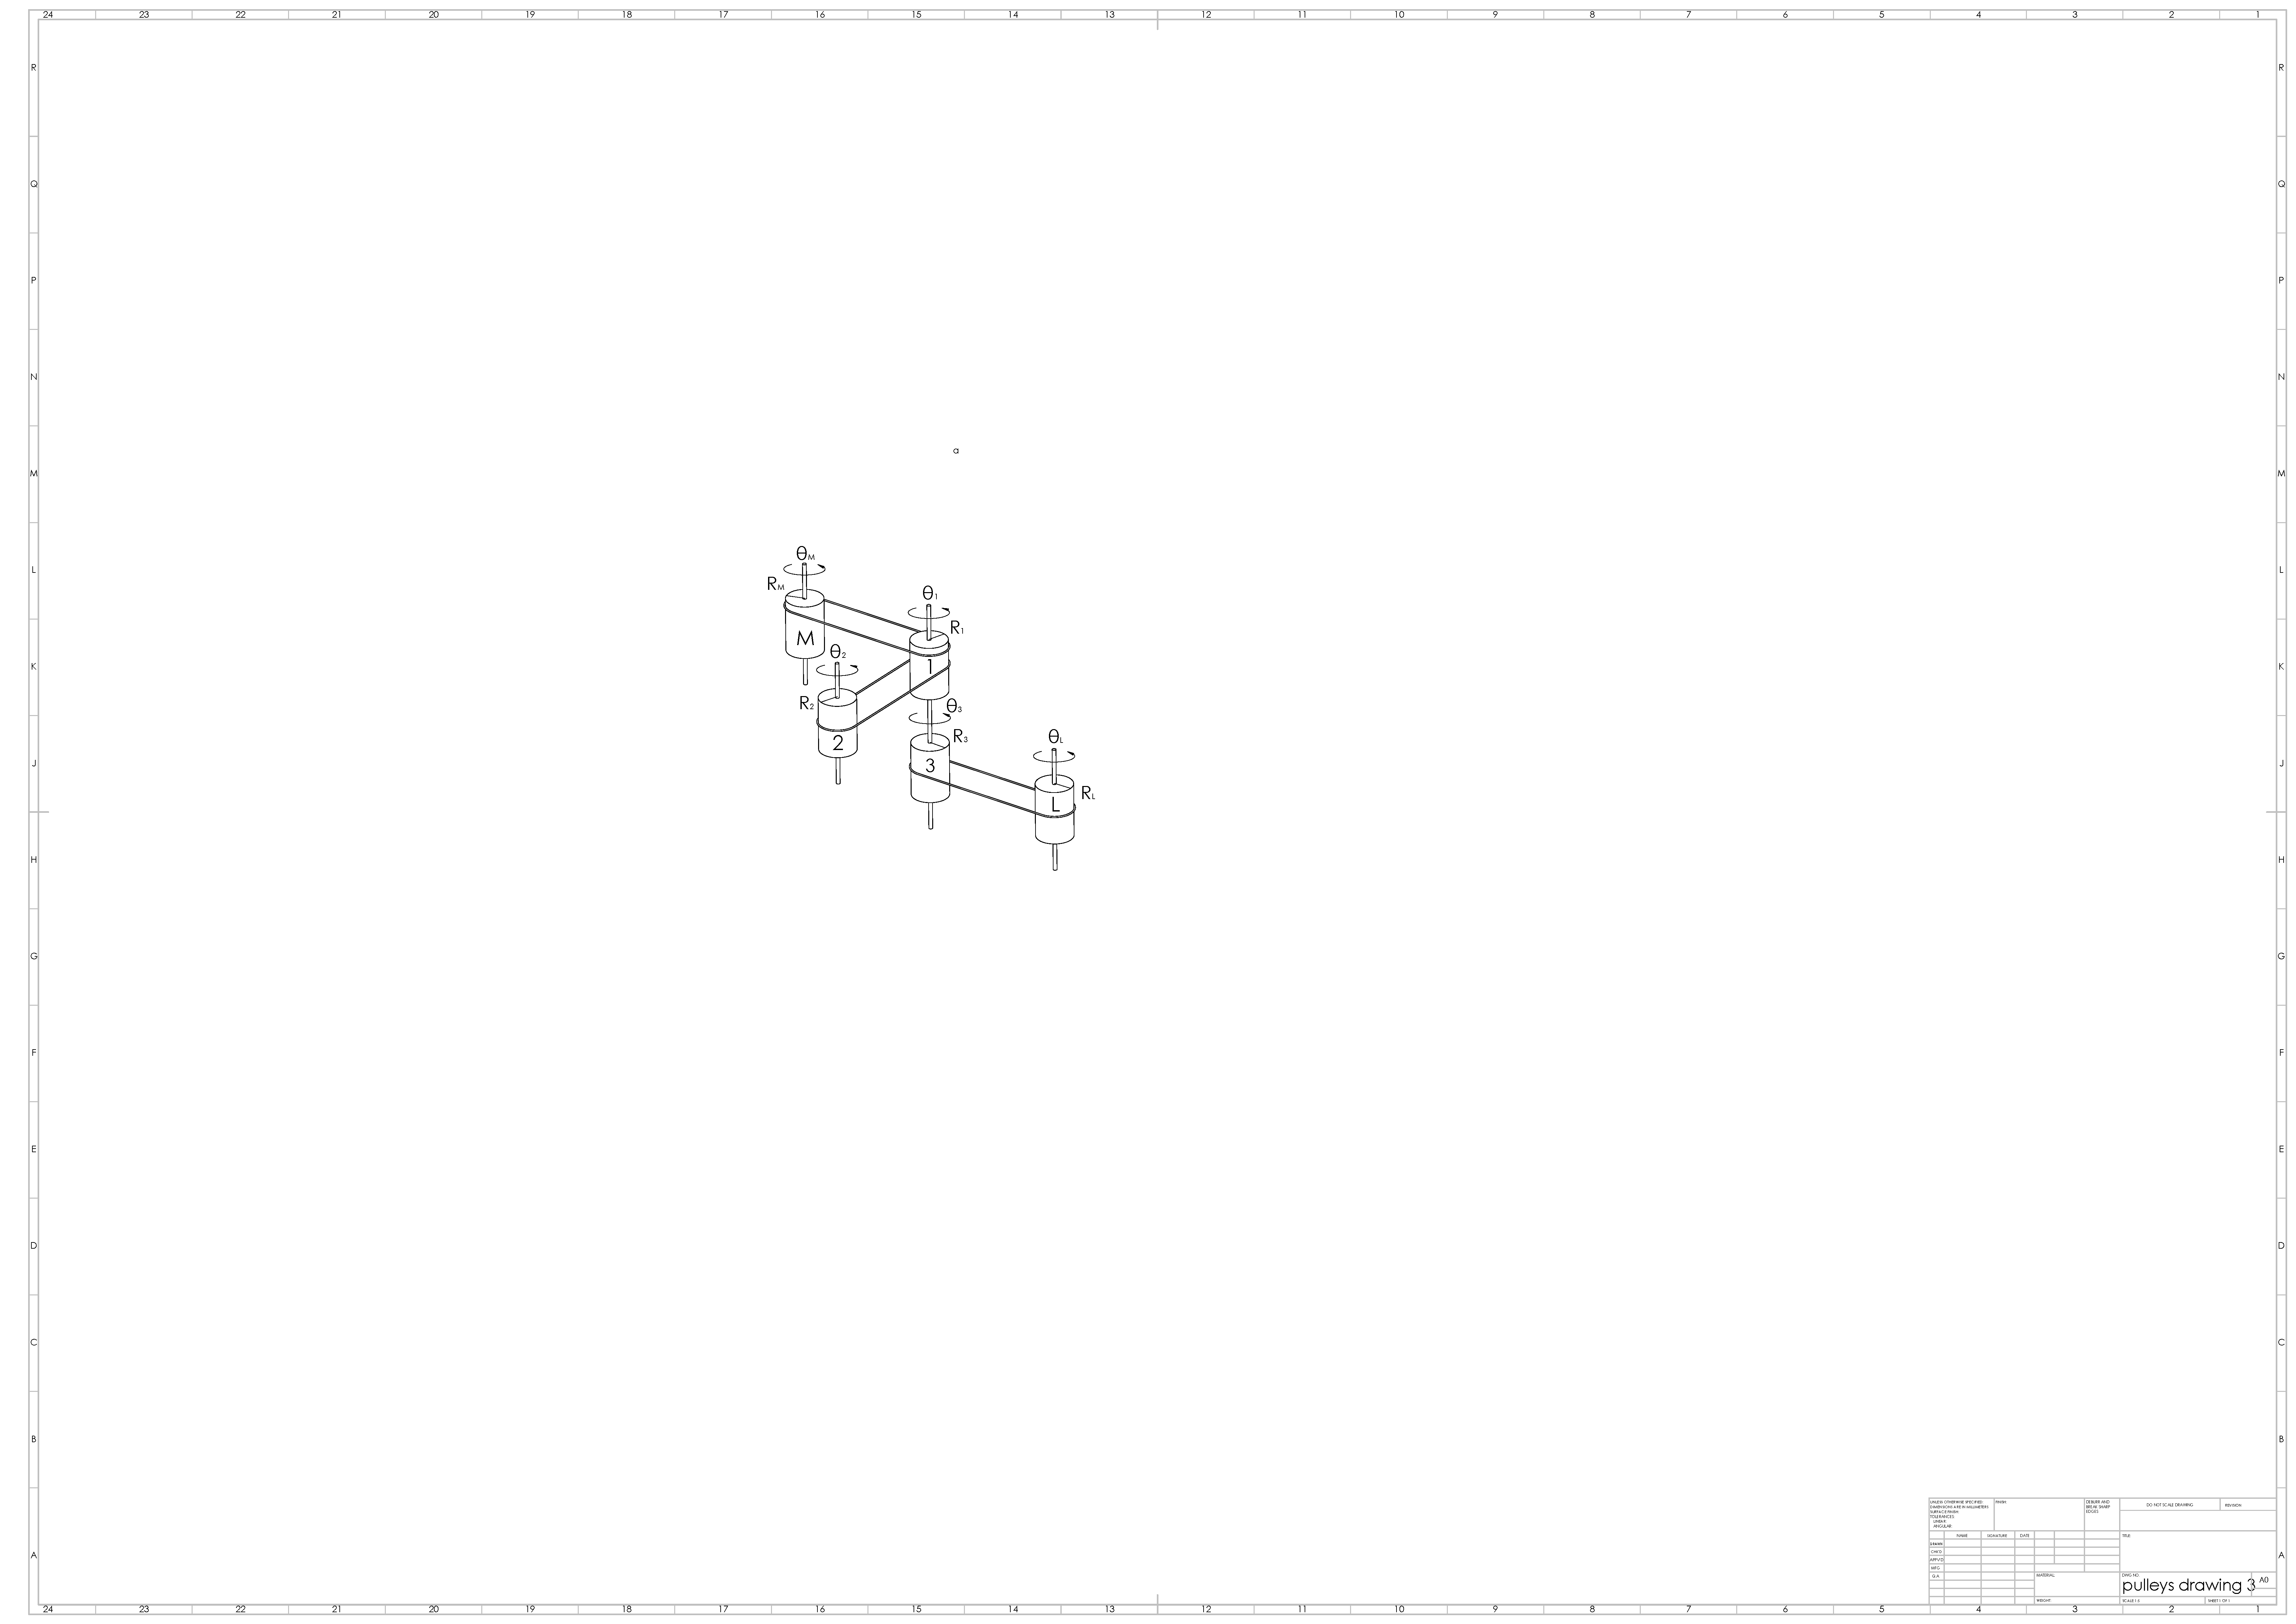
\includegraphics[width=\linewidth]{pulleys.pdf}
\caption{The pulley system of the Endowrist gripper modeled by equations (\ref{eq:dyn_1})-(\ref{eq:dyn_5}).}
\end{figure}

\begin{align}\label{eq:dyn_1}
J_m\ddot{{\theta}_m} + B_m \dot{{\theta}_m} + R_m T_{m1}(R_m {\theta}_m - R_1 {\theta}_1) = u_m
\end{align}
\begin{align}\label{eq:dyn_2}
J_L\ddot{{\theta}_L} + B_L \dot{{\theta}_L} + R_L T_{L3}(R_L {\theta}_L - R_3 {\theta}_3) = u_L
\end{align}
\begin{multline}\label{eq:dyn_3}
J_1\ddot{{\theta}_1}+ B_1 \dot{{\theta}_1} + R_1 T_{12}(R_1{\theta_1} - R_1{\theta}_3 - R_2{\theta_2})\\ = R_1 T_m(R_m{\theta}_m - R_1{\theta}_1)
\end{multline}
\begin{align}\label{eq:dyn_4}
J_2\ddot{{\theta}_2}+ B_2 \dot{{\theta}_2} + LF = R_2 T_{12}(R_1{\theta_1} - R_1{\theta}_3 - R_2{\theta_2})
\end{align}
\begin{multline}\label{eq:dyn_5}
J_3\ddot{{\theta}_3}+ B_3 \dot{{\theta}_3} + R_1 T_{12}(R_1{\theta_1} - R_1{\theta}_3 - R_2{\theta_2})\\ = R_3 T_{L3}(R_L{\theta}_L - R_3{\theta}_3)
\end{multline}

\todo{we should include what each variable corresponds to (T, J, R, F, theta)}

From equations \ref{eq:dyn_1}-\ref{eq:dyn_5} it is visible that this system can be converted to a linear state space model.
Moreover, simplifying the equations by replacing physical coefficients with general ones results in a 10th order state space model with 31 parameters.
This is the model we will perform parameter identification on.

\subsection{Parameter identification}
Parameter identification is performed using the Matlab parameter identification toolbox.
For us to tune the model parameters, it is necessary for us to perform experiments for input-output measurement datasets.

We do this by applying a known force $F$ to the gripper and measuring efforts on the actuators.
The goal here is to get a fully parametrized state space model which we can then use for grip force estimation with a Kalman filter.

At the time of wiriting this article, we are stil in the process of developing a full setup for fitting the state space model.
As a working model we are currently using an linear approximation based on torque and output downwards force measurement.

\begin{figure}
	\centering
	\begin{subfigure}{.45\linewidth}
		\centering
		\vspace{24pt}
		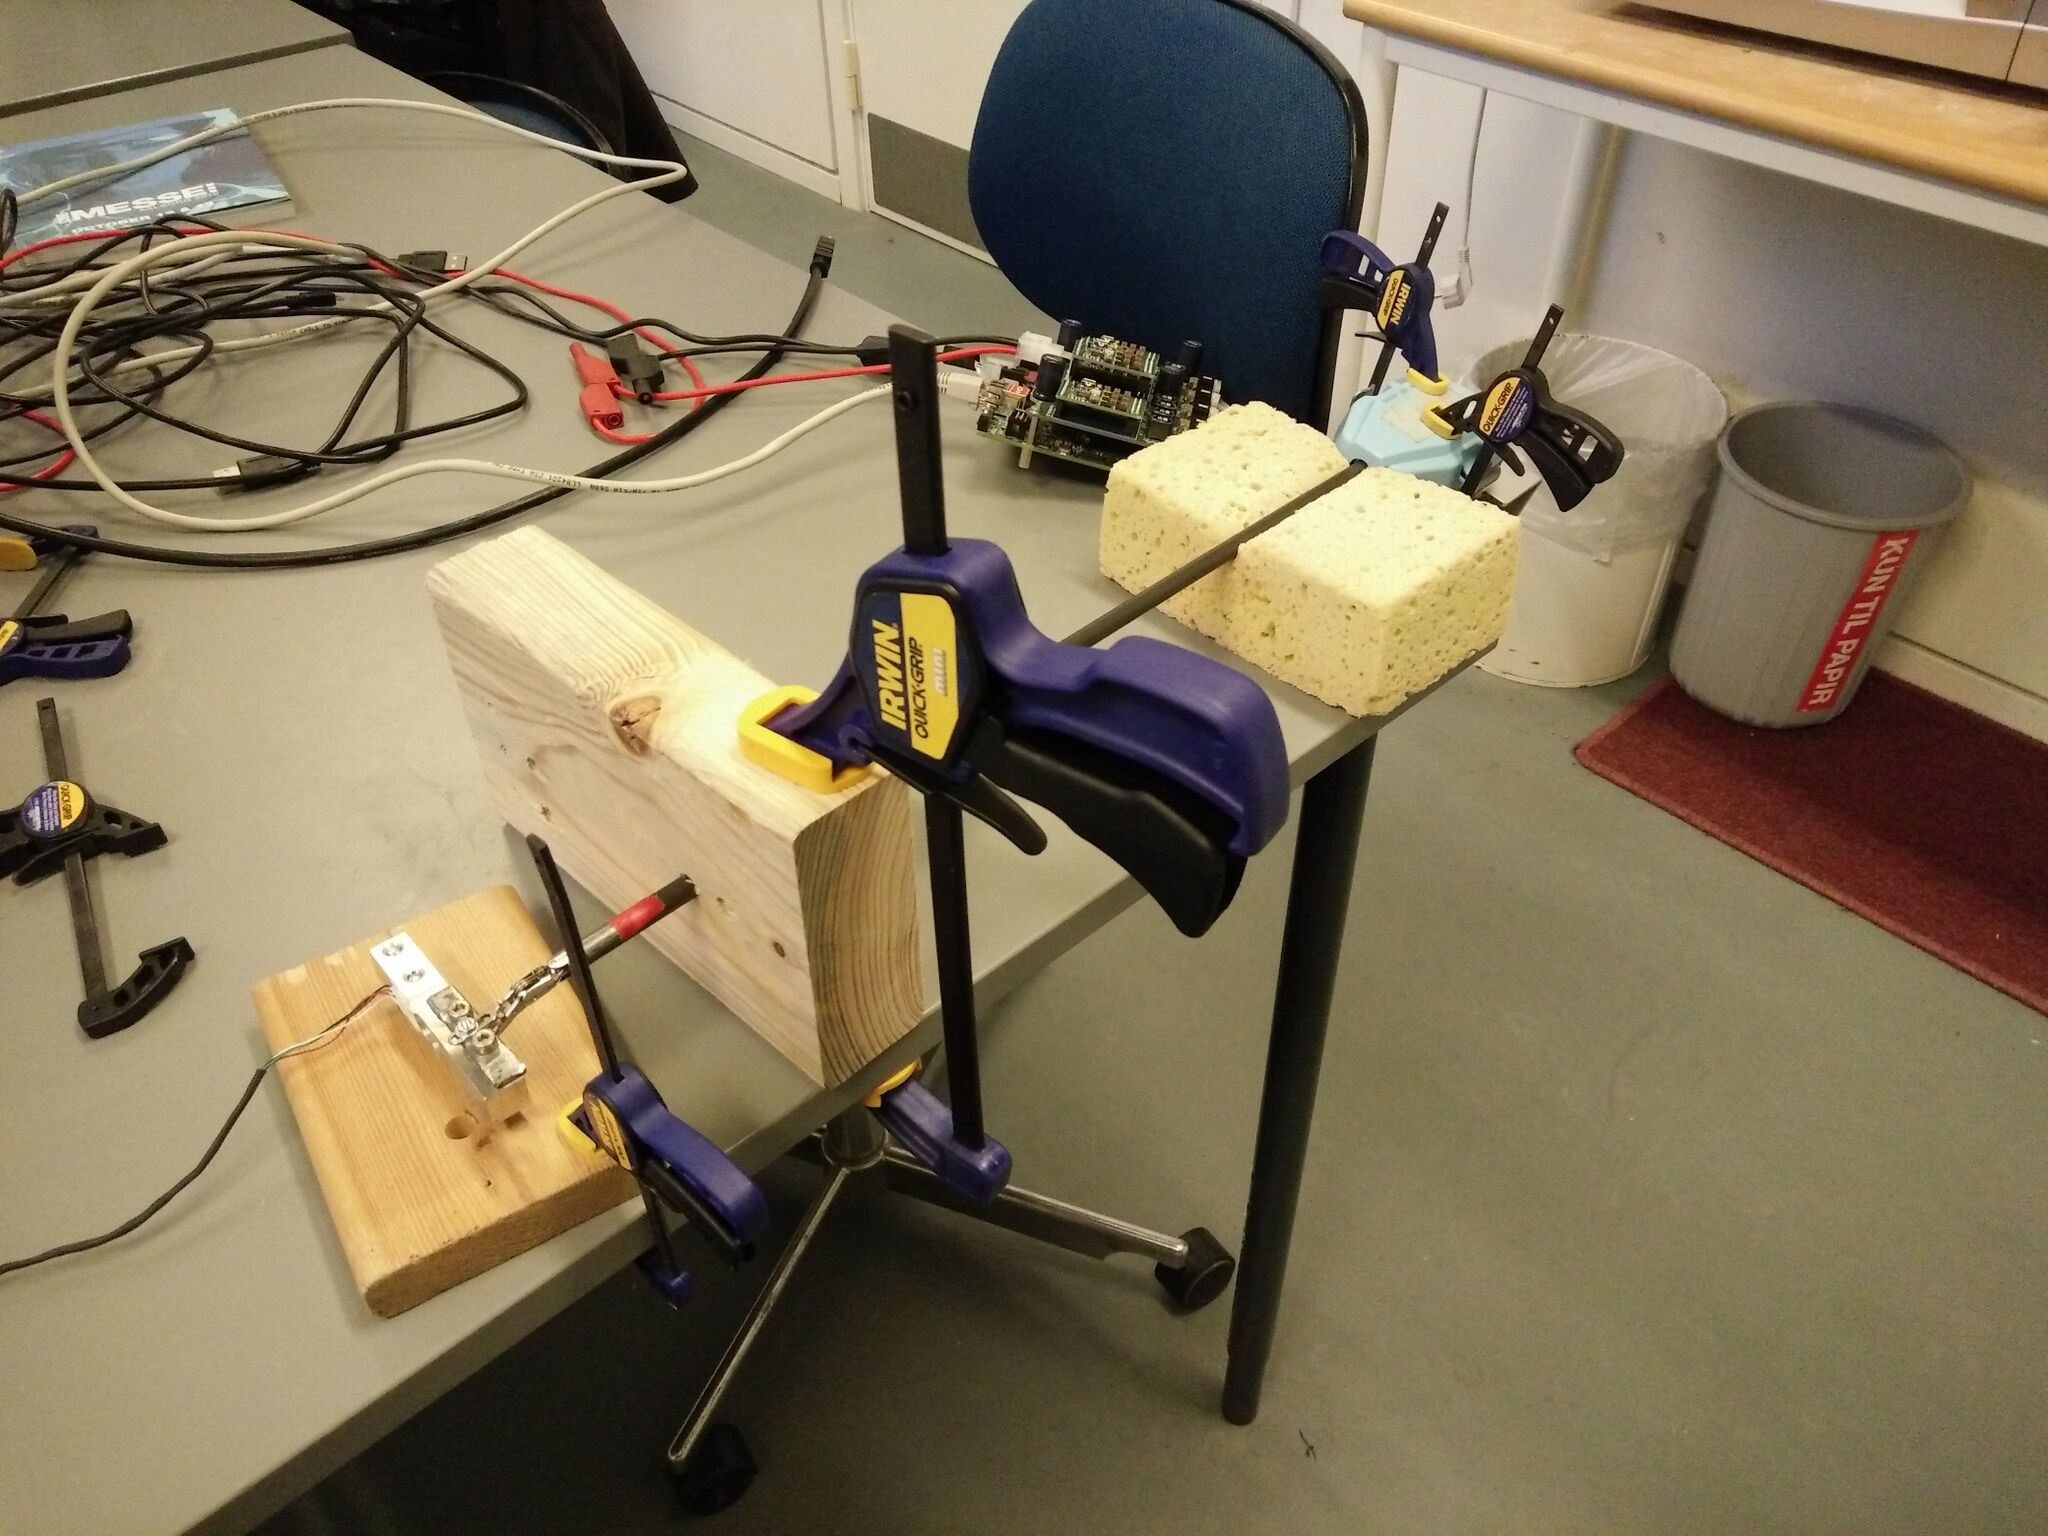
\includegraphics[width=\linewidth]{overall_force.jpg}
		\caption{The entire test setup. From the right, a scale for measuring the downwards force, a piece of wood for stiffening the Endowrist and keeping it it place and the Endowrist holder with motors.}
		\label{fig:entire_force_testsetup}
	\end{subfigure}
	\begin{subfigure}{.45\linewidth}
		\centering
		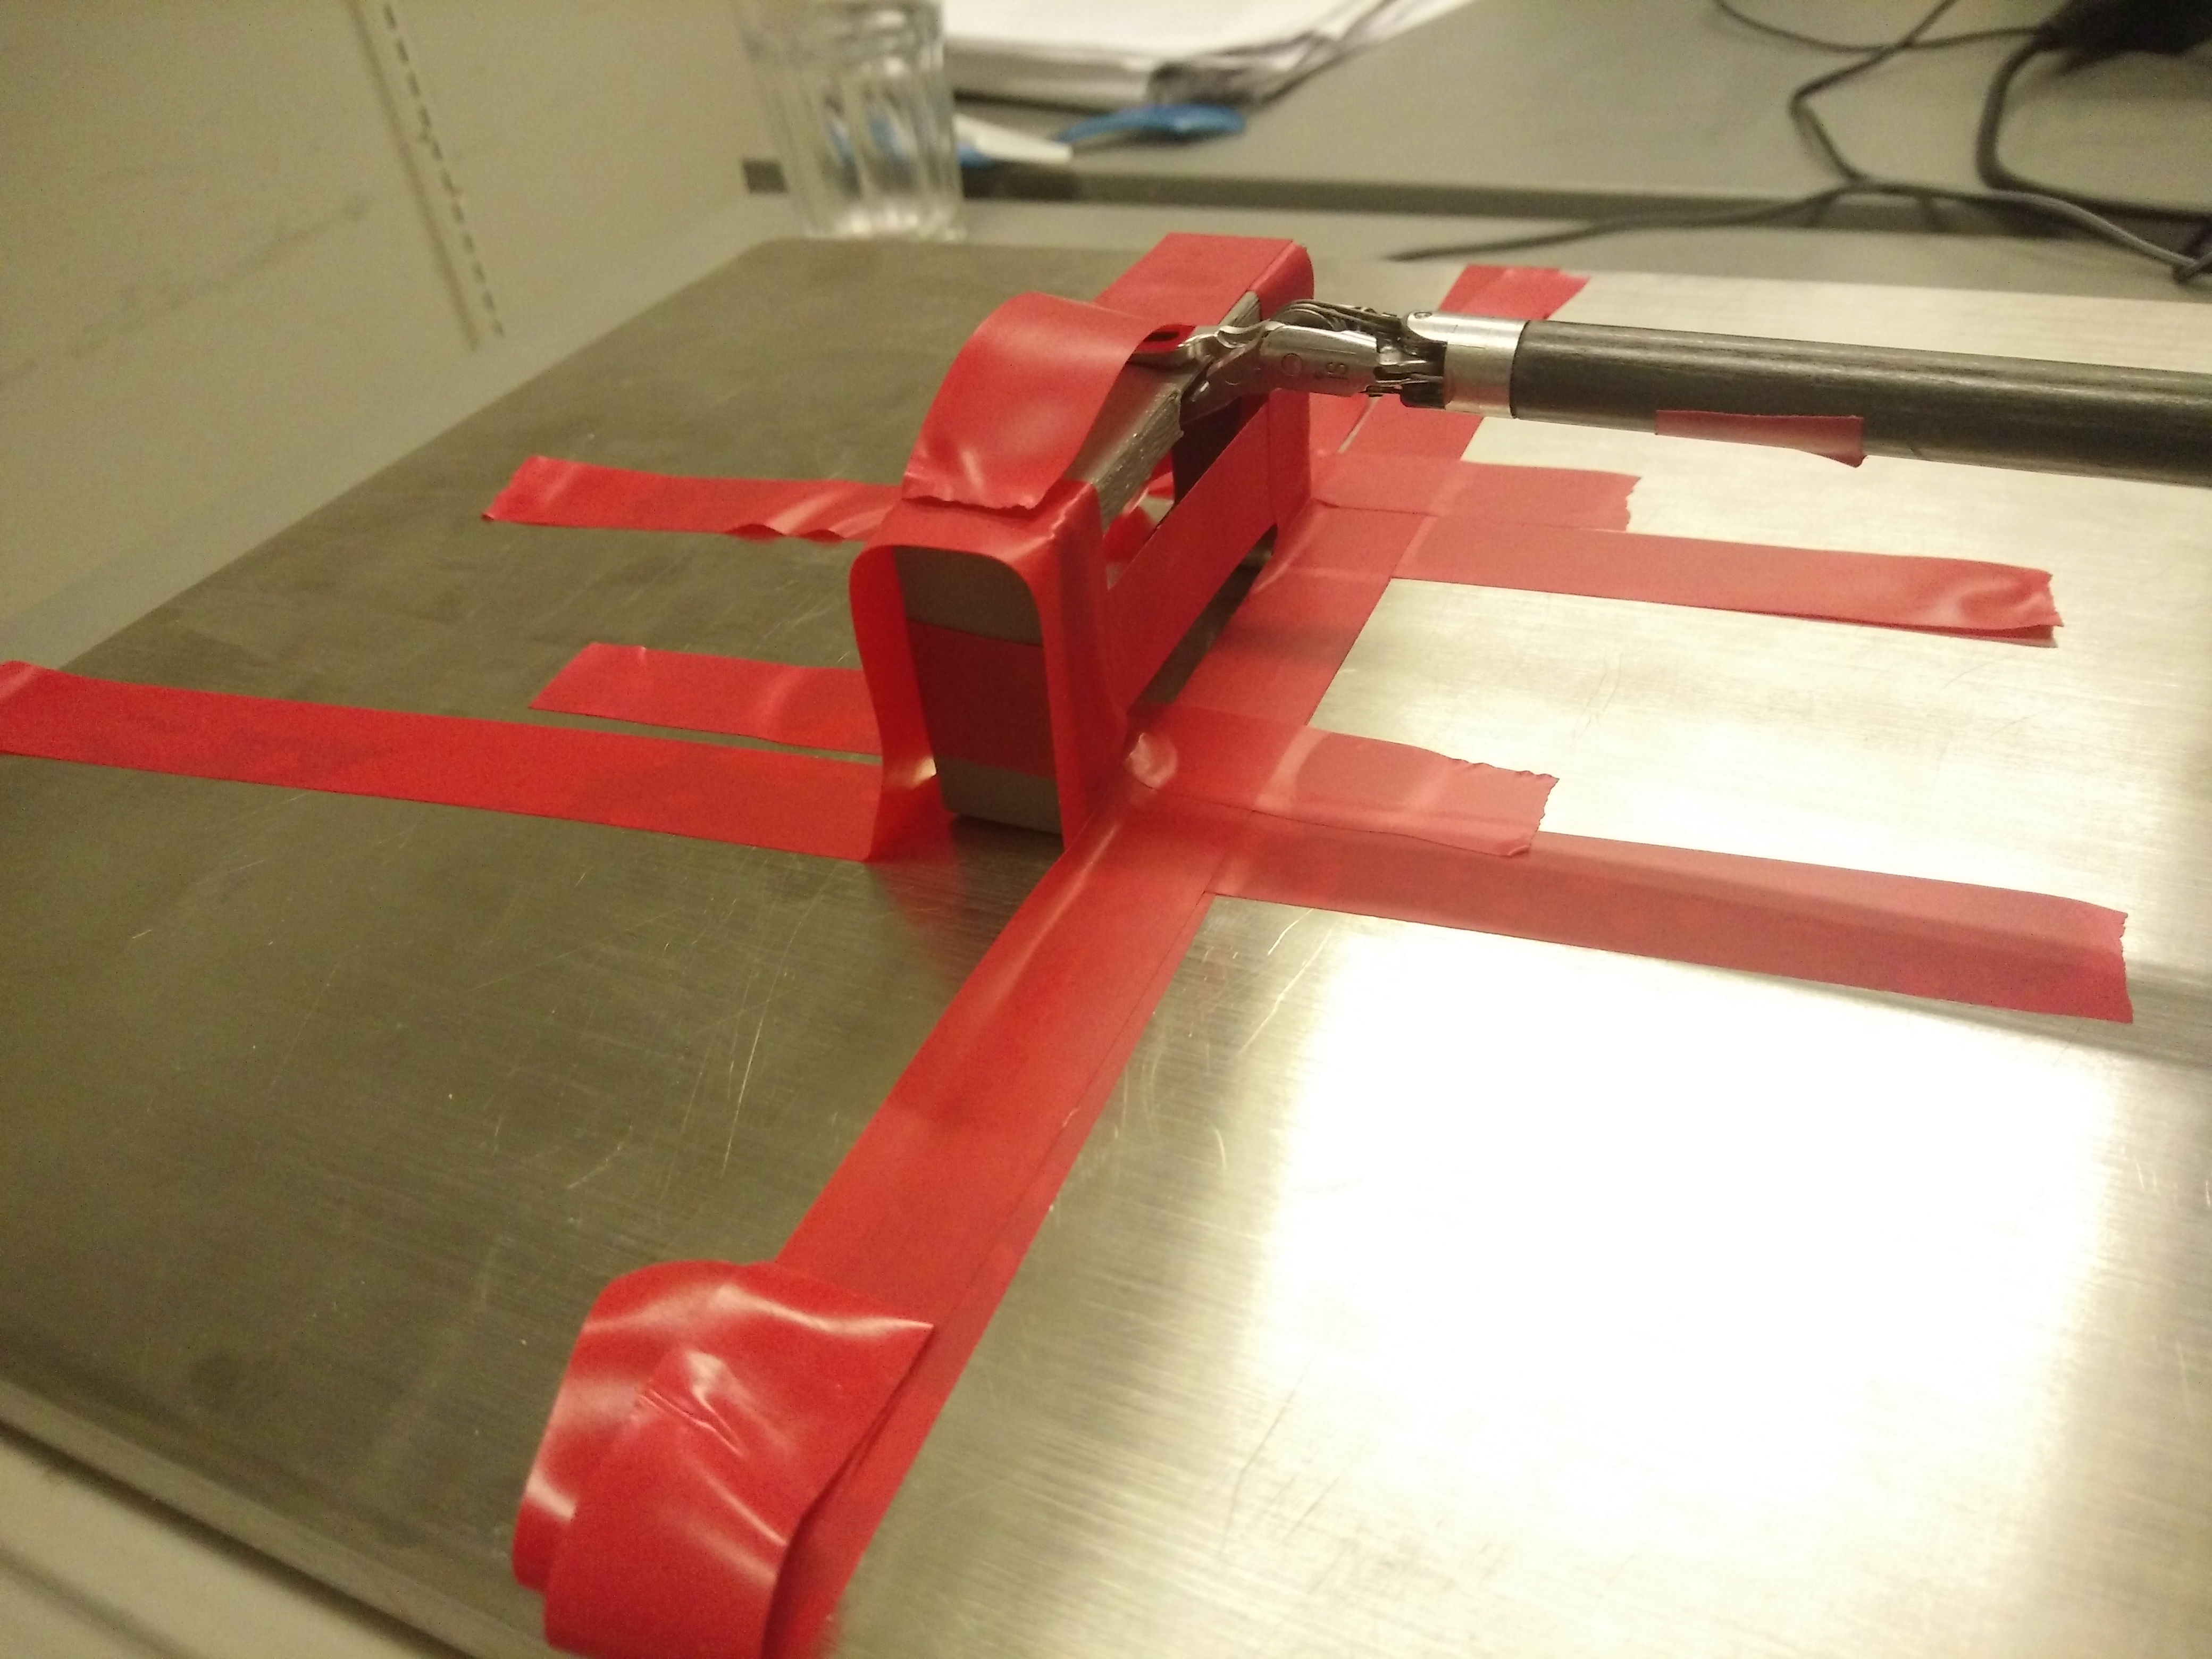
\includegraphics[width=\linewidth]{endeffector_force.jpg}
		\caption{A 3D printed case which made it possible to make an orthogonal force from the end-effector to the scale.}
		\label{fig:endeffector_force}
	\end{subfigure}
\caption{Test setup for the force estimation of the end-effector.}
\label{fig:Overview_force}
\end{figure}

A piecewise linear expression is made from the 340 mA sample and up and can be seen on \eqref{eq:linear_force_endo}.

\begin{equation}
\text{y} = 0.0028 \cdot \text{x} -0.8259 
\label{eq:linear_force_endo}
\end{equation} 
\section{Communication}

As mentioned before, the sbRIO board controls the motors in one arm. The desired positions of the motors are sent to the board from the computer using the Ethernet cable as well as the list of the enabled motors. For the computer to perform force estimation it needs to receive the list of the active motors as well as the position, velocity and effort for each of them.

It is said that the minimum refresh rate of haptic feedback is wildly debated to
be between 300 Hz and 600 Hz, but for a realistic force feedback it is commonly accepted
to be at least 1000 Hz\cite{coles2011role}. In order for the system to fulfill this requirement it is necessary that the communication between the sbRIO board and the computer at least match this frequency. That is why this project aims at getting as close as possible to 1000 Hz in the communication between the sbRIO and the computer.

In order to get the fastest communication it was decided to use UDP as it does not implement any reliability feature. Reliability in undesirable in our communication system as it would just lead to retransmitting obsolete data instead of transmitting the new one. Furthermore, most of the transport protocol implements features that improve long distance communication which would be superfluous in our test setup. 
 
In addition to the transport protocol, another factor that influence the speed of the communication is the size of the packets sent. To maximize the communication's speed, the size of the packets must be minimized while keeping the computation time as low as possible. As stated before, the packets exchanged between the computer and the sbRIO contain numerical values (positions, velocities and efforts) and booleans (active or enabled motors). The bitcode of the numerical values is interpreted as ASCII characters and the booleans are gathered in one byte which is also interpreted as a character. Those characters constitute the payload of the packets. As each numerical value is stored on 4 bytes, in the test setup the size of the payload sent by the computer to the sbRIO is be 17 bytes and the size of the payload sent by the sbRIO to the computer is 49 bytes.

To decrease the size of the packets even further the packets could be compressed however for most algorithms the size reduction is small for this amount of data and thus not worth the computation time.


\section{Results}

\subsection{Communication}

 It was stated before that the requirements for our system was to get to at least 600Hz and to reach 1000Hz if possible. As shown in Table \ref{tab:UDPMeasurements}, the connexion can go up to almost 1000Hz using UDP which fulfills the requirements. Nevertheless, the jitter should not be neglected as the frequency get closer to 1000Hz the jitter will be high compared to the period and may cause unexpected behaviour in real time operation. This issue will be further discussed in the next section. However, the data show a periodic disturbance in the system originating from the computer\todo{need some kind of graphical representation of that} which increases the jitter and delay. %Addictional safety precautions should be taken to prevent those behaviour.


\begin{table}[!t]
%\centering
  $\begin{tabular}{|c|c|c|c|c|c|}
    \hline
    \text{Delay} & \text{Frequency (Hz)} & \text{RTT* delay (ms)} & \text{Jitter} & \text{Error rate (\%)}\\
    \hline
    10ms & 86 & 1.8 & 2.7 & 0 \\
    \hline
    2ms & 447 & 2.1 & 3.5 & 1.2E-4 \\
    \hline
    0ms & 981 & 1.4 & 2.7 & 5.1E-5 \\
    \hline
  \end{tabular}$
  *Round Time Trip\\
  **The number of data set needs to be increased for the final version
  \caption{UDP**}
  \label{tab:UDPMeasurements}
\end{table}


% An example of a floating figure using the graphicx package.
% Note that \label must occur AFTER (or within) \caption.
% For figures, \caption should occur after the \includegraphics.
% Note that IEEEtran v1.7 and later has special internal code that
% is designed to preserve the operation of \label within \caption
% even when the captionsoff option is in effect. However, because
% of issues like this, it may be the safest practice to put all your
% \label just after \caption rather than within \caption{}.
%
% Reminder: the "draftcls" or "draftclsnofoot", not "draft", class
% option should be used if it is desired that the figures are to be
% displayed while in draft mode.
%
%\begin{figure}[!t]
%\centering
%\includegraphics[width=2.5in]{myfigure}
% where an .eps filename suffix will be assumed under latex,
% and a .pdf suffix will be assumed for pdflatex; or what has been declared
% via \DeclareGraphicsExtensions.
%\caption{Simulation results for the network.}
%\label{fig_sim}
%\end{figure}

% Note that the IEEE typically puts floats only at the top, even when this
% results in a large percentage of a column being occupied by floats.


% An example of a double column floating figure using two subfigures.
% (The subfig.sty package must be loaded for this to work.)
% The subfigure \label commands are set within each subfloat command,
% and the \label for the overall figure must come after \caption.
% \hfil is used as a separator to get equal spacing.
% Watch out that the combined width of all the subfigures on a
% line do not exceed the text width or a line break will occur.
%
%\begin{figure*}[!t]
%\centering
%\subfloat[Case I]{\includegraphics[width=2.5in]{box}%
%\label{fig_first_case}}
%\hfil
%\subfloat[Case II]{\includegraphics[width=2.5in]{box}%
%\label{fig_second_case}}
%\caption{Simulation results for the network.}
%\label{fig_sim}
%\end{figure*}
%
% Note that often IEEE papers with subfigures do not employ subfigure
% captions (using the optional argument to \subfloat[]), but instead will
% reference/describe all of them (a), (b), etc., within the main caption.
% Be aware that for subfig.sty to generate the (a), (b), etc., subfigure
% labels, the optional argument to \subfloat must be present. If a
% subcaption is not desired, just leave its contents blank,
% e.g., \subfloat[].


% An example of a floating table. Note that, for IEEE style tables, the
% \caption command should come BEFORE the table and, given that table
% captions serve much like titles, are usually capitalized except for words
% such as a, an, and, as, at, but, by, for, in, nor, of, on, or, the, to
% and up, which are usually not capitalized unless they are the first or
% last word of the caption. Table text will default to \footnotesize as
% the IEEE normally uses this smaller font for tables.
% The \label must come after \caption as always.
%
%\begin{table}[!t]
%% increase table row spacing, adjust to taste
%\renewcommand{\arraystretch}{1.3}
% if using array.sty, it might be a good idea to tweak the value of
% \extrarowheight as needed to properly center the text within the cells
%\caption{An Example of a Table}
%\label{table_example}
%\centering
%% Some packages, such as MDW tools, offer better commands for making tables
%% than the plain LaTeX2e tabular which is used here.
%\begin{tabular}{|c||c|}
%\hline
%One & Two\\
%\hline
%Three & Four\\
%\hline
%\end{tabular}
%\end{table}


% Note that the IEEE does not put floats in the very first column
% - or typically anywhere on the first page for that matter. Also,
% in-text middle ("here") positioning is typically not used, but it
% is allowed and encouraged for Computer Society conferences (but
% not Computer Society journals). Most IEEE journals/conferences use
% top floats exclusively.
% Note that, LaTeX2e, unlike IEEE journals/conferences, places
% footnotes above bottom floats. This can be corrected via the
% \fnbelowfloat command of the stfloats package.

\section{Discussion}
Safety and "compression"
\section{Conclusion}
The conclusion goes here.




% conference papers do not normally have an appendix


% use section* for acknowledgment
\section*{Acknowledgment}


The authors would like to thank...





% trigger a \newpage just before the given reference
% number - used to balance the columns on the last page
% adjust value as needed - may need to be readjusted if
% the document is modified later
%\IEEEtriggeratref{8}
% The "triggered" command can be changed if desired:
%\IEEEtriggercmd{\enlargethispage{-5in}}

% references section

% can use a bibliography generated by BibTeX as a .bbl file
% BibTeX documentation can be easily obtained at:
% http://mirror.ctan.org/biblio/bibtex/contrib/doc/
% The IEEEtran BibTeX style support page is at:
% http://www.michaelshell.org/tex/ieeetran/bibtex/
%\bibliographystyle{IEEEtran}
% argument is your BibTeX string definitions and bibliography database(s)
%\bibliography{IEEEabrv,../bib/paper}
%
% <OR> manually copy in the resultant .bbl file
% set second argument of \begin to the number of references
% (used to reserve space for the reference number labels box)
\medskip
\bibliographystyle{IEEEtran}
\bibliography{Bibliography}

%\begin{thebibliography}{1}

% \bibitem{IEEEhowto:kopka}
% H.~Kopka and P.~W. Daly, \emph{A Guide to \LaTeX}, 3rd~ed.\hskip 1em plus
%   0.5em minus 0.4em\relax Harlow, England: Addison-Wesley, 1999.

%\bibitem{RIGSP}
%Giulianotti, P. C., Coratti, A., Angelini, M., Sbrana, F., Cecconi, S.,
%et al., \emph{Robotics in General Surgery Personal Experience in a Large Community Hospital}\hskip 1em plus
%  0.5em minus 0.4em\relax Archives of Surgery: pp. 777-784.

%\bibitem{EOFGFF}
%H.~Kopka and P.~W. Daly, \emph{Effects of haptic and graphical force feedback on teleoperated palpation}\hskip
%  0.5em minus 0.4em\relax  Robotics and Automation: pp. 677 - 682.

%  \todo{not sure on the "pp"}

%\end{thebibliography}




% that's all folks
\end{document}
